\documentclass[12pt]{article}

\usepackage{amsmath}
\usepackage[margin = 1in]{geometry}
\usepackage{booktabs}
\usepackage{natbib}
\usepackage{graphicx}
\usepackage{float}
\usepackage{setspace}
\usepackage{caption}
\captionsetup[table]{skip=10pt}
\usepackage[colorlinks=true, citecolor=blue]{hyperref}


\begin{document}


\begin{titlepage}
  \begin{center}
      \vspace*{1cm}
      \Huge
      \textbf{Analysis of Men's Tennis 2022 Grand Slam Performance}

      \large
      \vspace{0.5cm}
       Exploration of likelihood factors affecting Men's Tennis Grand Slam outcomes.
           
      \vspace{1.5cm}

      \textbf{Kaitlyn Shevlin}
     
      \vspace{0.8cm}
        
       \Large    
      Department of Statistics\\
      University of Connecticut\\
      Storrs, CT\\
           
  \end{center}
\end{titlepage}

\doublespace{}

\begin{abstract}

This research investigates the factors that lead to winning matches in men's 
singles Grand Slam tournaments. Utilizing data from 509 matches in 2022, 
the aim is to discover if a higher ATP ranking is indicative of the outcome of 
match. In addition, both non-specific and specific player analysis will be 
conducted to explore singular factors such as court type, as well as a comination 
of factors such as if winning the first set, along with a higher ATP ranking, will 
lead to a win. This research will examine particular factors as well as new combinations
of elements that affect play over the year of 2022.\\

\noindent{\sc Keywords}:
Exploratory analysis; Tennis Grand Slams; Sports Data; Statistics.
\end{abstract}


\section{Introduction}
\label{sec:intro}

Tennis has a long and distinguished history, gaining popularity in
19th century France. The sport has developed into a world-class sport
drawing a large fan base all across the world. The Mens Tennis Grandslam 
Tournaments are notorious events that feature the world's best tennis players. 
There are four Grand Slams- the Australian Open, the French Open, Wimbledon, 
and the U.S. Open, spanning from January to September. Extensive research has 
been completed on modeling future and past player performance in conjunction 
with the improvement of game tracking technologies.

Exploratory analysis about tennis is important for metrics on both the
courts and matches as well as the players. Many predictions are made well 
before the Grand Slams are played, mainly based off metric and trends. 
Looking at past ATP rankings of players going into the tournament, and then 
examinging the outcome of the match, will reveal how ATP translates to the 
matches and if the player with the higher ATP going into the match is more 
likely to win.

Tennis is unique in that several court surfaces are used- clay, grass, and hard 
surfaces, that players must adapt to. Each court type has various advantages and
disadvantages around play and maintence, in addition to player specific preferences.
The French open is played on clay courts which can be characterized by high bounce
but overall a slow surface which is best for baseline players. Rafeal Nadal is 
considered "the King of Clay," which can be attributed to him growing up in Spain
where clay courts are predominant. His specific skillset also aligns well with the
features of clay courts. Wimbledon takes place on grass courts which are the opposite
to clay, in that it is the fastest surface with a low bounce. Roger Federer excelled
here as it favors players with large serves and those who prefer to play close to the
net. Hard courts are utilzed for the U.S. and Australian Opens, characterized by high,
predictable bounces and medium speed. 

Prior research has been done regarding top ranked tennis players, both males and 
females. Much analysis surrounding top performers throughout the years and the 
relationshp between the changes in ATP rankings have been researched. As this 
dataset includes statistics from 2022, there is less specific research conducted.

The Association of Tennis Professionals (ATP) is the world's governing
body for men's tennis whereas the Women's Tennis Associaton (WTA)
is the world's governing body in women's tennis. Both the ATP and
WTA have computerized tennis rankings for singles and doubles players.
There is no systematic ranking for mixed doubles as of yet. These
rankings are based on points earned in one's best 19 events, 16 for women,
as this number is capped at 19 to prevent someone who plays in more tournaments
per year to be at an advantage. Points awarded for Grand Slams are greater
than points for other tournaments and events \citet{Nag2022Tennis}.

The following table shows the ATP ranking points awarded for each type of match.

\begin{table}[ht]
  \caption{ATP ranking points table}
  \label{tab:ATP}
\centering
\begin{tabular}{
  |p{\dimexpr.285\linewidth-2\tabcolsep-1.3333\arrayrulewidth}
  |p{\dimexpr.065\linewidth-2\tabcolsep-1.3333\arrayrulewidth}
  |p{\dimexpr.065\linewidth-2\tabcolsep-1.3333\arrayrulewidth}
  |p{\dimexpr.065\linewidth-2\tabcolsep-1.3333\arrayrulewidth}
  |p{\dimexpr.065\linewidth-2\tabcolsep-1.3333\arrayrulewidth}
  |p{\dimexpr.065\linewidth-2\tabcolsep-1.3333\arrayrulewidth}
  |p{\dimexpr.065\linewidth-2\tabcolsep-1.3333\arrayrulewidth}
  |p{\dimexpr.065\linewidth-2\tabcolsep-1.3333\arrayrulewidth}
  |p{\dimexpr.065\linewidth-2\tabcolsep-1.3333\arrayrulewidth}
  |p{\dimexpr.065\linewidth-2\tabcolsep-1.3333\arrayrulewidth}
  |p{\dimexpr.065\linewidth-2\tabcolsep-1.3333\arrayrulewidth}
  |p{\dimexpr.065\linewidth-2\tabcolsep-1.3333\arrayrulewidth}|
  }
  \hline
Tournament Level & W & F & SF & QF & R16 & R32 & R64 & R128 & Q & Q3 & Q2\\ 
  \hline
Grand Slam & 2000 & 1200 & 720 & 360 & 180 & 90 & 45 & 10 & 25 & 16 & 8 \\ 
\hline
ATP 1000 - 96 Draw & 1000 & 600 & 360 & 180 & 90 & 45 & 25 & 10 & 16 &  & 8\\ 
\hline
ATP 1000 - 48/56 Draw & 1000 & 600 & 360 & 180 & 90 & 45 & 10 &  & 25 &  & 16\\
\hline
ATP 500 - 48 Draw & 500 & 300 & 180 & 90 & 45 & 20 &  &  & 10 &  & 4\\ 
\hline
ATP 500 - 32 Draw & 500 & 300 & 180 & 90 & 45 &  &  &  & 20 &  & 10\\ 
\hline
ATP 250 - 48 Draw & 250 & 150 & 90 & 45 & 20 & 10 &  &  & 5 &  & 3\\
\hline
ATP 250 - 32 Draw & 250 & 150 & 90 & 45 & 20 &  &  &  & 12 &  & 6\\
\hline
ATP Challenger Tour 125 & 125 & 75 & 45 & 25 & 10 & & & & & & \\
\hline
ATP Challenger Tour 110 & 110 & 65 & 40 & 20 & 9 & 5 & & & & & \\
\hline
ATP Challenger Tour 100 & 100 & 60 & 35 & 18 & 8 & 5 & & & & & \\
\hline
ATP Challenger Tour 90 & 90 & 55 & 33 & 17 & 8 & 5 & & & & & \\
\hline
ATP Challenger Tour 80 & 80 & 48 & 29 & 15 & 7 & 3 & & & & & \\
\hline
ITF World Tennis Tour $25,000 / $25,000+H & 20 & 12 & 6 & 3 & 1 & & & & & & \\
\hline
ITF World Tennis Tour $15,000 / $15,000+H & 10 & 6 & 4 & 2 & 1 & & & & & & \\
  \hline
\end{tabular}
\end{table}

This goal of this research is to investigate if ATP is a significant factor
in predicting the outcome of the match. Prior research has revealed weaknesses 
in the ATP ranking system which has its basis rooted in points. Other ranking 
systems such as UTR, do not deal with points, instead it utilizes algorithms to 
assess player performance in relation to their most recent matches \citet{Bodo2022Rankings}. 
Keeping this in mind, this exploration will see how heavily and accurately ATP 
ranking played a role in the outcome of the match. 



\section{Data}
\label{sec:data}

The data is acquired from tennis.data.co.uk which provides detailed historical 
and recent sports data \citep{TennisBetting}. The site compiles the information 
from the sources ATPtennis.com, ATP Tour Rankings and Results Page, and Sony 
Ericsson WTA Tour. The dataset for this research includes figures from the four 
men's tennis Grand Slam tournaments in 2022. The data provides many specific 
factors that play a role in matches as well as an abundance of results which will 
aid in the analysis and regression.

The element descriptions are clearly labeled on the site as follows: 

ATP = tournament number for men

WTA = tournament number for women

Location = venue of tournament

Tournament =  name of tournament (four major Grand Slams)

Series = name of ATP tennis series

Court = type of court (indoors or outdoors)

Surface = type of surface (clay, hard, carpet, or grass)

Round = round of match

Best of = maximum number of sets playable in a match (5 for mens) 

Winner = match winner 

Loser = match loser

WRank = ATP entry ranking of match winner as of the start of the tournament

LRank = ATP entry ranking of match loser as of the start of the tournament

WPts = ATP entry points of match winner as of the start of the tournament

LPts = ATP entry points of match loser as of the start of the tournament

W1 = number of games won in 1st set by match winner

L1 = number of games won in 1st set by match loser

W2 = number of games won in 2nd set by match winner

L2 = number of games won in 2nd set by match loser

W3 = number of games won in 3rd set by match winner

L3 = number of games won in 3rd set by match loser

W4 = number of games won in 4th set by match winner

L4 = number of games won in 4th set by match loser

W5 = number of games won in 5th set by match winner

L5 = number of games won in 5th set by match loser

Wsets = number of sets won by match winner

Lsets = number of sets won by match loser

Comment = comment on the match (completed, won through retirement of loser, or walkover)\\

The data provides number of games won in each set for match winner and loser which will 
aid in the examination of predicting match winner by success in the first game as well 
as the relationships between ATP ranking of the players coming into the match and the outcome 
of the match. No visualizations are provided but clear descriptives are stated.


\section{Methods}
\label{sec:meth}


I will be using logistic regresion which is a classification algorithm. The logistic 
function 
\begin{equation}
  \label{eq:logreg}
    \ \sigma(t) = \frac{1}{1 + e^-t}
\end{equation}
  
The regression will explore the relationships between factors as well as interactions 
between factors such as WRank and LRank to find if coming in with a better ranking is 
indicative of the outcome.






\section{Results}
\label{sec:results}

To find if the ATP ranking of the players entering the match have an impact, I created a new 
variable called upset which gives the output "Predicted" if the winner of the match had a higher 
ATP ranking coming in; and "Upset" if the loser of the match had the higher ranking. The graph 
below shows the count of each.

\begin{table}[ht]
  \caption{Count of Outcome}
  \label{tab:upset}
\centering
\begin{tabular}{rr}
  \hline
Outcome & Count \\
  \hline
Predicted & 141 \\
Upset & 367 \\
  \hline
\end{tabular}
\end{table}


As seen in the table above, many upsets occur, leading us to first believe that ATP ranking is not 
a good predictor.


\begin{figure} 
  \centering
  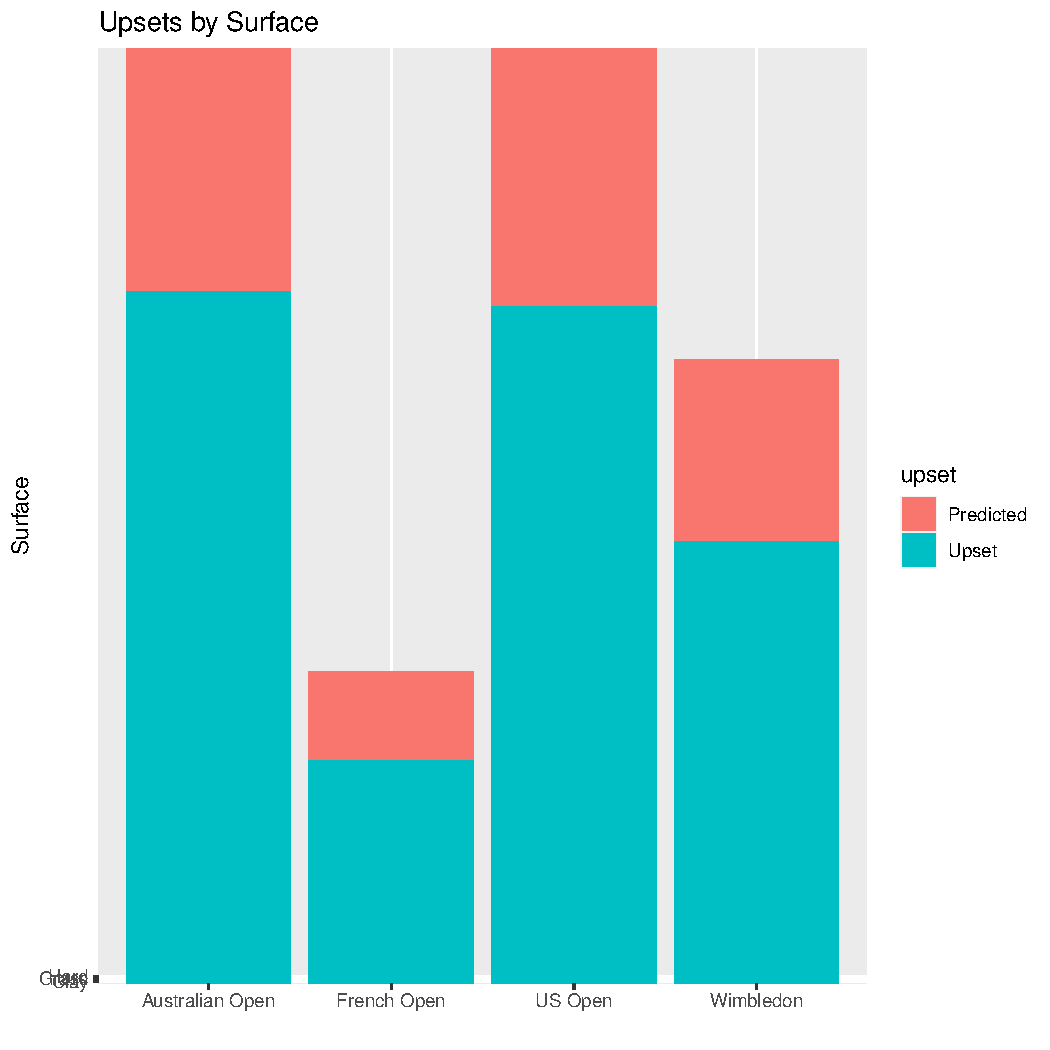
\includegraphics[width=\textwidth]{surfaceoutcome.pdf}
  \caption{Outcomes by Surface.}
 \label{fig:upsets}
\end{figure}


\section{Dicussion}
\label{sec:discussion}

This current study is only utilizing data from 2022 so for future studies, 
a wider variety of newer data can be used to further analyze trends and changes over time.
The main contributions of this study are to show that ATP ranking is not completely accurate 
or a good predictor of the outcome of Men's Grand Slam tennis matches. It is worth pursuing 
further analysis and exploration of other ranking systems that accurately portray a player's 
standings and a way to improve upon ATP's points focused approach.



\bibliography{refs}
\bibliographystyle{chicago}

\end{document}